\section{Pregunta N$^{\circ}$13\qquad Leon Alonzo Terrones Caccha}

\begin{frame}
    \begin{enumerate}\setcounter{enumi}{12}
        \item


              Para la función
              \begin{math}
                  f\left(t\right)=
                  \sqrt{t}
              \end{math}
              use diferencias divididas para construir el polinomio
              de Newton de grado $2$ para los puntos $t_{0}=0$,
              $t_{1}=1$ y $t_{2}=3$.
    \end{enumerate}

    \begin{solution}
    \[
\begin{array}{cccccc}
x_0=0 & y_0=0 \\
    &     & 1 \\
x_1=1 & y_1=1 &             & \frac{\sqrt{3}-3}{6}\\
    &     & \frac{\sqrt{3}-1}{2}\\
x_2=3 & y_2=\sqrt{3}
\end{array}
\]
\end{solution}
\end{frame}
\begin{frame}
        \begin{figure}[ht!]
            \centering
            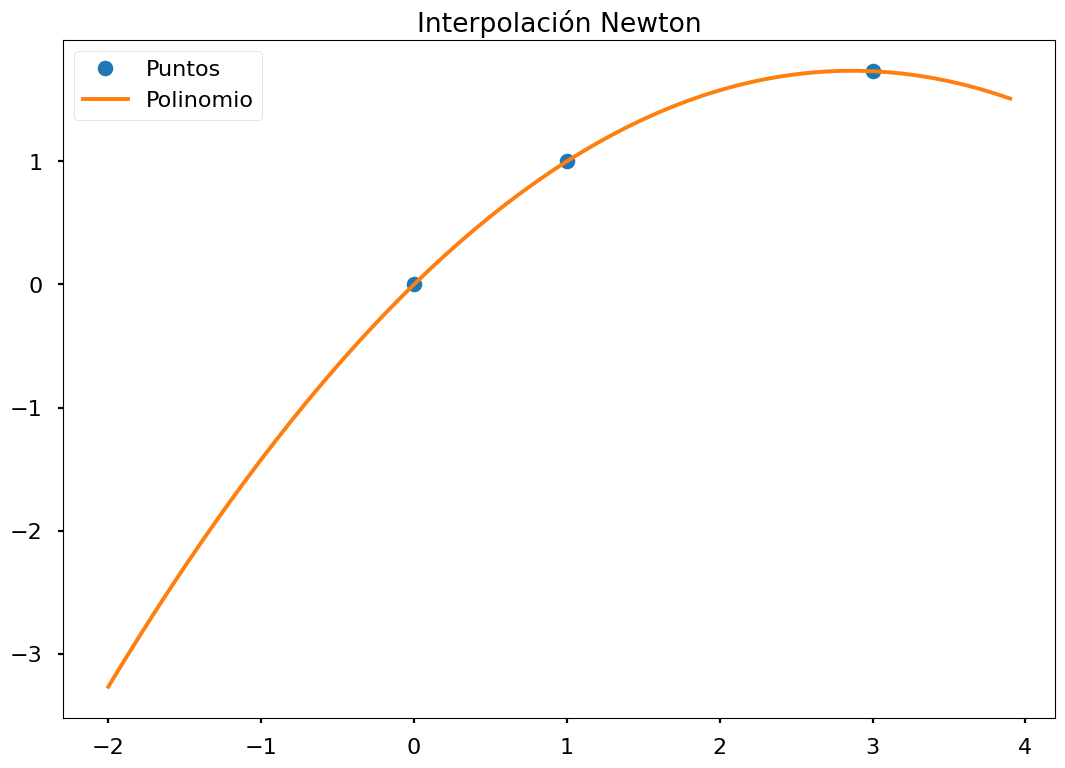
\includegraphics[width=.6\paperwidth]{P13-2.png}
        \end{figure}
\end{frame}